\documentclass[final]{beamer}
\usetheme{SIB}
\usepackage[orientation=portrait,size=a2,scale=1.4,debug]{beamerposter}
\usepackage[absolute,overlay]{textpos}
\usepackage{alltt} 
\setlength{\TPHorizModule}{1cm}
\setlength{\TPVertModule}{1cm}

\newcommand{\green}[1]{\textcolor{green!60!black}{#1}}
\newcommand{\red}[1]{\textcolor{red!60!black}{#1}}
\newcommand{\blue}[1]{\textcolor{blue!60!black}{#1}}

\title{pfsearch next generation:\\ accelerated search of PROSITE profiles}
\author{\textbf{Thierry Schuepbach}$^{1,3}$, Marco Pagni$^1$, Alan Bridge$^2$, Lydie Bougueleret$^2$, Ioannis Xenarios\,$^{1,2}$, \textbf{Lorenzo Cerutti}\,$^{2}$}
\institute{$^1$Vital-IT group, SIB Swiss Institute of Bioinformatics, Amphipole, UNIL-Sorge, CH-1015 Lausanne\\
           $^2$Swiss-Prot group, SIB Swiss Institute of Bioinformatics, CMU, Rue Michel-Servet 1, CH-1211 Geneva\\
           $^3$Molecular Modeling group, SIB Swiss Institute of Bioinformatics, Amphipole, UNIL-Sorge, CH-1015 Lausanne}
\footer{\texttt{http://web.expasy.org/pftools/\#pfsearchV3}\hskip1em\raisebox{-0.3cm}{
\includegraphics[width=0.034\linewidth]{QR.png}}}
\date{}

\begin{document}
\begin{frame}{} 

\begin{textblock}{19.5}(1,9.4)
\begin{block}{Summary}
The PROSITE (http://prosite.expasy.org) resource provides a rich and well annotated source of signatures in the form of generalized profiles that allow protein domain detection and functional annotation. One of the major limiting factors in the application of PROSITE in genome and metagenome annotation pipelines is the time required to search protein sequence databases for putative matches. We describe an improved and optimized implementation of the PROSITE search tool \emph{pfsearch} that is intended to address this limitation.
\end{block}

\begin{block}{An heuristic for pfsearch}
A major reduction in the execution time of sequence database searches can be achieved by introducing an heuristic pre-filter that selects candidate sequences. We implemented an heuristic for generalized profiles, named \emph{prfh}:
\begin{itemize}
\item each position $i$ of the profile and $j$ of the sequence we define a score $S(i,j)$:
\begin{equation*}
  S(i,j) = \max\left\{     \begin{array}{l}     S(i-1, j-1) + M(i,a_j) \\     0     \end{array}     \right. \label{eq:01}
\end{equation*}
    where $M(i,a_j)$ is the match score read at position $i$ of the profile matrix table for residue $a_j$ observed at position $j$ of the sequence. 
\item only the maximal scoring diagonal $S(i,j)$ is kept for every position $j$ of the sequence. All maxima are then summed to form the final heuristic score ($H_{score}$).
\begin{equation*}
  H_{score}=\sum_j\bigl(\max_{i}S(i,j)\bigr) \label{eq:02}
\end{equation*}
\end{itemize}
\end{block}
\begin{block}{Calibration of the heuristic for PROSITE profiles}
The $H_{score}$ distribution linearly correlates with the raw score distribution obtained using the standard pfsearch ($R^2 \approx 0.9$ on average). We use this property to determine the appropriate $H_{score}$ cutoffs with respect to the normalized score cutoffs of each calibrated profile:
\begin{itemize}
\item randomly sample 200 sequences belonging to the original seed alignment (re-sampling if their number is $<$200);
\item generate a set of artificially mutated sequences based on the sampled sequences, including indels, at various PAM distances sharing from ~40\% to ~85\% sequence identity with their source;
\item score the sequences with both the standard profile scoring method and the heuristic;
\item calculate the regression line on the lower 5\% quantile of the heuristic score distribution using the quanteg R package, and use it to obtain the heuristic cutoffs corresponding to the standard profile cutoffs. (NB: The regression on a low quantile ensures a minimal loss of true positive sequences)
\end{itemize}
\vskip-2.5em
\begin{columns}[c]
    \begin{column}{0.3\paperwidth}
    \begin{figure}[!tpb]%figure1
    \centerline{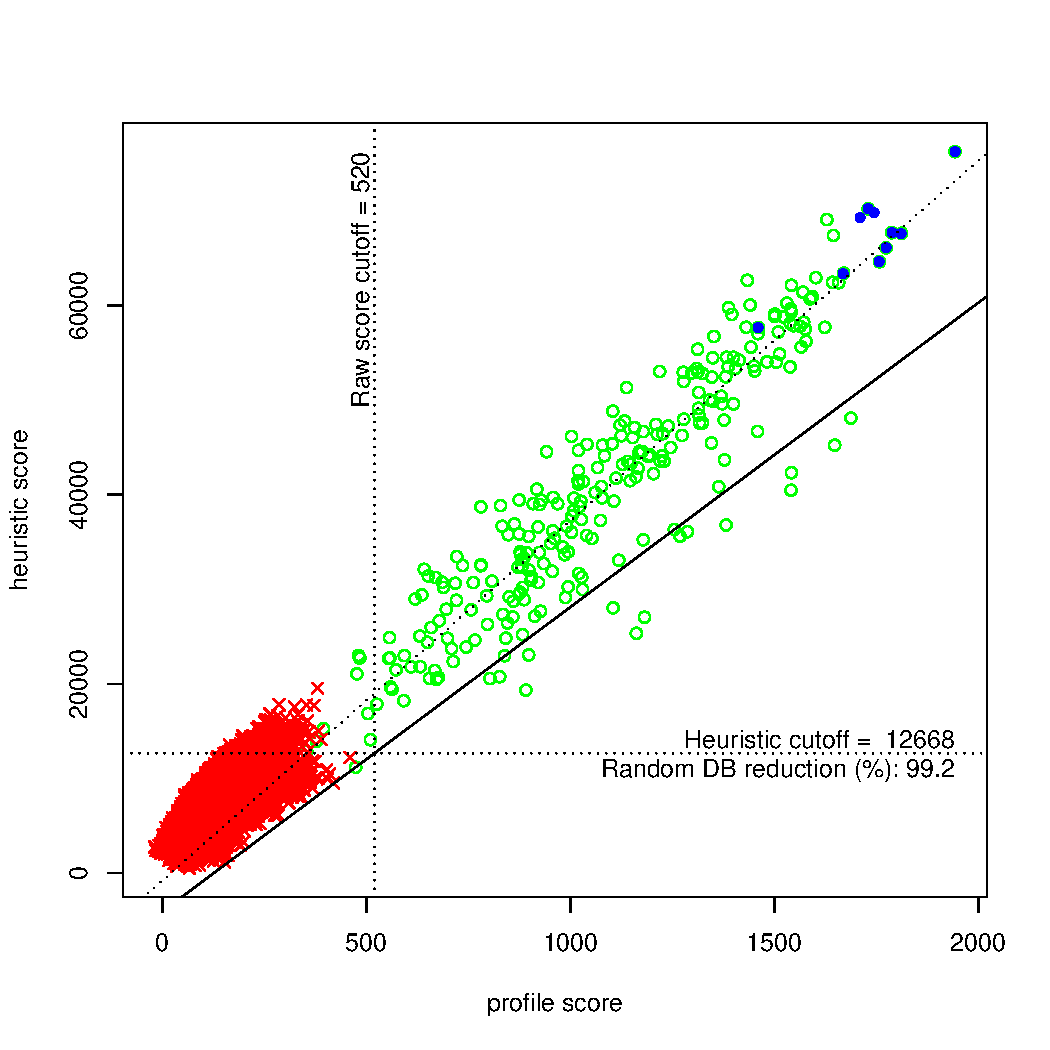
\includegraphics[angle=0,width=0.83\hsize]{figure1.pdf}}
    \end{figure}
    \end{column}
    \hskip-1em
    \begin{column}{0.2\paperwidth}
Example: estimation of the $H_{score}$ cutoff from the regression line of the lower 5\% quantile (black line) for profile CYTOCHROME\_B5\_2 ($R^2$=0.9):\\
    \vskip1em
    \begin{tabular}{cl}
      \blue{$\bullet$} & sequences from seed \\
      & alignment;\\ 
      \red{$\times$}   & shuffled sequences; \\
      \green{$\circ$}  & simulated sequences. \\
    \end{tabular}
    \end{column}
\end{columns}
\end{block}
\end{textblock}

\begin{textblock}{19.3}(21.8,9.4)
\begin{block}{The new H\_score keyword}
We introduced a new keyword H\_score to in PROSITE profiles to inform the program of the heuristic cutoffs. The keyword do not interfere with the previous version of the \emph{pfsearch} program.
    \centerline{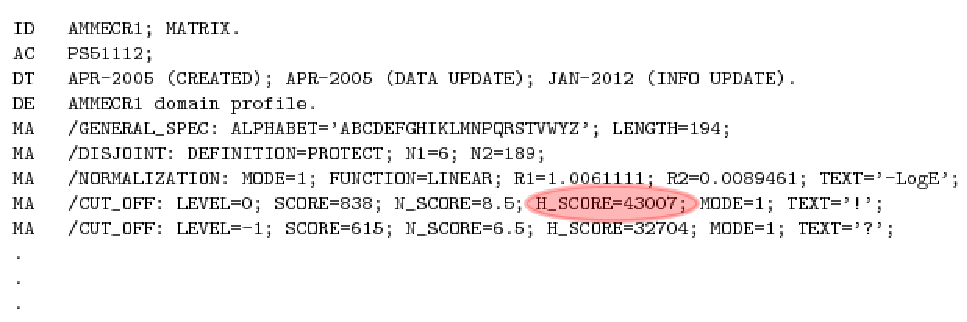
\includegraphics[angle=0,width=1.00\hsize]{prf_synt.pdf}}
\end{block}

\begin{block}{Software optimization}
Pfsearch has been rewritten and optimized in C from the original Fortran:
\begin{itemize}
\item we entirely reformatted the memory structure to allow vectorization;
\item high level assembly code (intrinsic functions) was used to enforce the SSE 2 and SSE 4.1 instruction sets;
\item added multi-thread support.
\end{itemize}
On a single core, the new software implementation runs 2$\times$ faster than the original Fortran. This acceleration scales up with multi-threading: on a dual hyperthreaded quad-core machine we measured an average 10-fold improvement. The sequence database was also indexed to avoid repeated disk access for sequence scanning, particularly useful for repeated calls when searching multiple profiles. 
\end{block}

\begin{block}{Performance}
The performance obtained by combining the developed heuristic and the software optimization has been measured for the 904 PROSITE profiles, for which we were able to fix the H\_score cutoff, against 16,544,936 UniProtKB sequences (5,358,014,649 residues).  All measures have been obtained using a dual hyperthreaded quad-core Intel workstation.
\vskip 1em
{\scriptsize
\begin{table}
\begin{tabular}{r||c|c}
\hline
& Mean& Median\\
\hline
TP recovery                    & 99.6\%  & 99.9\% \\
Database reduction (heuristic) & 96.7\%  & 99.1\% \\
& & \\
\multicolumn{1}{l||}{Search time/profile:} & & \\ 
pfsearchV3 &  98 sec & 73 sec \\
pfsearch on Vital-IT cluster & 5-10 mins$^{(*)}$ & -\\
standard pfsearch & 3 hours$^{(*)}$ & -\\
\hline
\end{tabular}
\end{table}
}
\vskip 1em
$^{(*)}$ estimated time for a profile of length 120.\\
NB: most of the missing TP matches correspond to fragment sequences.
\newline
\end{block}

\begin{block}{Conclusion}
By combining the heuristic with our code optimization we achieved a 100x fold increase in the speed of pfsearch on average on a modern workstation. For example the human proteome can be searched with the totality of the PROSITE profile models in less than 4 hours and this time can be drastically reduced on machines with a large number of CPU cores and/or computer clusters.
\end{block}
\end{textblock}

\end{frame}

\end{document}
